\documentclass[12pt]{article}

\usepackage[T1]{fontenc}
\usepackage[utf8]{inputenc}
\usepackage[a4paper,margin=1in]{geometry}
\usepackage{setspace}
\usepackage{microtype}
\usepackage{amsmath,amssymb,amsfonts,bm}
\usepackage{amsthm}
\usepackage{newtxtext,newtxmath}
\usepackage{booktabs}
\usepackage{threeparttable}
\usepackage{tabularx}
\usepackage{array}
\usepackage{longtable}
\usepackage{makecell}
\usepackage{float}
\usepackage{placeins}
\usepackage{pdflscape}
\usepackage{graphicx}
\usepackage{caption}
\usepackage{titlesec}
\usepackage{enumitem}
\usepackage{fancyhdr}
\usepackage[round,authoryear]{natbib}
\usepackage[hidelinks]{hyperref}
\usepackage{url}
\usepackage{indentfirst}
\doublespacing
\setlength{\parindent}{1.15em}
\setlength{\parskip}{0pt}
\captionsetup{font={small,stretch=1.0},labelfont=bf}
\renewcommand{\arraystretch}{1.08}
\setlength{\LTcapwidth}{\textwidth}
\setlist{nosep,leftmargin=1.2em}
\emergencystretch=3em
\hyphenpenalty=10000
\exhyphenpenalty=10000
\sloppy
% Applied Economics heading hierarchy: first-level bold; second-level bold italic; third-level italic.
\titleformat{\section}{\normalfont\bfseries\normalsize}{\thesection}{0.75em}{}
\titleformat{\subsection}{\normalfont\bfseries\itshape\normalsize}{\thesubsection}{0.75em}{}
\titleformat{\subsubsection}{\normalfont\itshape\normalsize}{\thesubsubsection}{0.75em}{}
\titlespacing*{\section}{0pt}{1.4ex plus .2ex}{0.8ex}
\titlespacing*{\subsection}{0pt}{1.2ex plus .2ex}{0.6ex}
\titlespacing*{\subsubsection}{0pt}{1.0ex plus .2ex}{0.5ex}

\pagestyle{fancy}
\fancyhf{}
\fancyhead[C]{\small Release-Ladder GDP Nowcasting}
\fancyfoot[C]{\thepage}
\renewcommand{\headrulewidth}{0.4pt}
\renewcommand{\footrulewidth}{0pt}

\hfuzz=1000pt

\newcolumntype{Y}{>{\raggedright\arraybackslash}X}
\newcolumntype{L}[1]{>{\raggedright\arraybackslash}p{#1}}
\newcolumntype{C}[1]{>{\centering\arraybackslash}p{#1}}
\newcommand{\code}[1]{\texttt{#1}}
\newcommand{\Arel}{\mathrm{A}}
\newcommand{\Srel}{\mathrm{S}}
\newcommand{\Trel}{\mathrm{T}}
\newcommand{\Mrel}{\mathrm{M}}
\newcommand{\Exact}{\mathrm{exact}}
\newcommand{\Pseudo}{\mathrm{pseudo}}
\newcommand{\dSA}{\Delta^{\Srel,\Arel}}
\newcommand{\dTS}{\Delta^{\Trel,\Srel}}
\newcommand{\dMT}{\Delta^{\Mrel,\Trel}}
\newtheorem{proposition}{Proposition}

\title{Release-ladder real-time nowcasting of US GDP:\\
Exact-vintage evidence on point forecasts, density forecasts, and revision risk}
\author{%
\begin{minipage}{0.95\textwidth}
\centering
Minh Ha Quang\\[0.75em]
National Economics University, Vietnam\\[0.5em]
Corresponding author: Minh Ha Quang,
\href{mailto:haminh1092005@gmail.com}{haminh1092005@gmail.com},
ORCID: \href{https://orcid.org/0009-0009-0143-5042}{0009-0009-0143-5042}
\end{minipage}
}
\date{}

\begin{document}
\maketitle
\thispagestyle{fancy}

\begin{abstract}
\noindent
This article studies US real GDP nowcasting as a release-ladder problem rather than a single final-vintage prediction problem. For each reference quarter, the operational target is the next official GDP estimate observed by real-time users: advance, second, or third release; mature releases are retained only for robustness. The article constructs exact-vintage information sets aligning monthly indicator availability, GDP release timing, Bureau of Economic Analysis (BEA) / National Income and Product Accounts (NIPA) targets, historical GDP vintages, and Survey of Professional Forecasters (SPF) coverage over 2005Q1--2024Q4. Results are stage-dependent. Before the advance release, SPF is the strongest point benchmark, with exact-timing root mean squared error (RMSE) of 2.225. After an official estimate is public, no-revision becomes the hard institutional benchmark, with RMSE of 0.570 before the second release and 0.362 before the third. Release-revision state-space models do not deliver universal point-RMSE dominance. Their contribution is clearest for density forecasts, intervals, and adjacent-revision risk. The indicator-revision state-space model has the lowest continuous ranked probability score (CRPS) for the third-release point target. Nowcasting systems should therefore be evaluated against the official release stage faced by the user.
\end{abstract}

\noindent\textbf{Keywords:} GDP nowcasting; real-time data; data revisions; macroeconomic forecasting; state-space models.

\noindent\textbf{JEL classification:} C32; C53; E17; E32.

\section{Introduction}
\label{sec:introduction}

Macroeconomic decisions are made before national-account data are complete. Early GDP estimates rely on incomplete source data and later revisions can change real-time forecasting conclusions \citep{landefeld2008,croushorestark2001,croushore2011}. Nowcasting must therefore align the target, forecast origin, and admissible monthly information \citep{giannone2008,banbura2013,bok2018}.

US real GDP makes this alignment problem explicit. The Bureau of Economic Analysis (BEA) publishes advance, second, and third estimates before later mature revisions \citep{beaNIPA2026,philadelphiaRTDSM2026}. Before the first official estimate, the Survey of Professional Forecasters (SPF) is the natural external point benchmark; after an official estimate is public, no-revision becomes the relevant institutional benchmark \citep{spf2026,anesti2022,mankiwshapiro1986}.

This distinction matters empirically because a later-release forecast is not simply a more informed version of the pre-advance nowcast. It is partly a forecast of how the statistical agency will revise an already released estimate. A model can therefore be useful in two different ways: by improving the conditional mean of the next release, or by quantifying the probability distribution of the next revision around a strong carry-forward benchmark. A design that evaluates only one GDP vintage risks mixing these two tasks.

This article reframes GDP nowcasting as a release-ladder problem. It constructs advance, second, third, and mature targets; aligns each target with checkpoint-specific real-time information; and evaluates point loss, density loss, adjacent-revision risk, mature-target robustness, and numerical reliability. The results are conservative: SPF wins before the advance release, no-revision wins before the second and third releases, and release-aware state-space models contribute mainly through uncertainty and revision-risk assessment. The article therefore argues for stage-specific evaluation rather than a single champion nowcasting model. The contribution is applied rather than purely methodological: it asks which benchmark a real-time user should beat at each public release stage.

Three implementation choices follow. Release timing is part of the empirical object; flexible models face professional, institutional, regression, factor, and state-space benchmarks; and point accuracy is separated from distributional usefulness. This separation is essential for later releases, where no-revision can be nearly optimal for the conditional mean even though users still need probabilities for revision size and direction.


\section{Literature review}
\label{sec:literature}

\subsection{Nowcasting, data flow, and operational targets}

Modern GDP nowcasting infers current-quarter activity from incomplete monthly indicators, publication lags, and ragged-edge data \citep{giannone2008,banbura2013,bok2018}. The release-ladder perspective adds target alignment: a forecast before the advance release is not the same object as a forecast made after the advance estimate is public. Real-time studies show that both the data vintage and the evaluation target must match the forecast origin \citep{croushorestark2003,croushore2011}.

Most operational systems track monthly releases, but that focus does not by itself specify which GDP release is being forecast. The target definition is therefore as important as the information set.

\subsection{Dynamic factor and mixed-frequency methods}

Dynamic factor models (DFMs) summarize macroeconomic panels with common activity signals \citep{forni2000,stockwatson2002,bai2002}. State-space and mixed-frequency methods handle missing observations, temporal aggregation, and monthly-quarterly timing \citep{doz2011,marianomurasawa2003,schorfheide2015}. MIDAS and bridge specifications provide regression-based competitors \citep{ghysels2007,marcellinoschumacher2010,kuzin2011}. Related extensions include unrestricted MIDAS, missing-data and quasi-maximum-likelihood factor estimation, density-combination nowcasting, and vintage-aware VAR/revision forecasting \citep{foroni2015,banburamodugno2014,doz2012,aastveit2014,clementsgalvao2008,clementsgalvao2012,clementsgalvao2013,kishorkoenig2012}. This article uses those tools, but its contribution is the release-specific target and information-set design rather than a new generic DFM estimator.

The comparison is intentionally plural: factor and state-space models handle ragged edges, MIDAS and bridge equations are familiar applied benchmarks, and no-revision is the relevant institutional rule once a preliminary GDP estimate exists.

\subsection{Real-time vintages and GDP revisions}

The real-time data literature shows that using revised data as if they were available in real time can distort forecast evaluation \citep{croushorestark2001,croushorestark2003,koenig2003}. GDP revisions add a second issue: preliminary estimates may contain news or noise, and release histories can be forecast objects in their own right \citep{mankiwshapiro1986,jacobsvannorden2011,anesti2022}. This article embeds that perspective in a US release-ladder evaluation where the benchmark changes once a preliminary official estimate becomes public.

The design also separates mature GDP from the headline targets. Mature values matter for robustness, but they are not the same object as the next public release observed by a forecaster.

\subsection{Forecast evaluation, density scoring, and the gap filled here}

Density forecasts are evaluated with proper scores such as log score and the continuous ranked probability score (CRPS) \citep{gneitingraftery2007,gneiting2007}. Loss comparisons and model-confidence diagnostics discipline interpretation when later-release RMSE gaps are small \citep{dieboldmariano1995,giacominiwhite2006,hansen2011}. Nested-model and instability-oriented comparisons provide complementary forecast-evaluation diagnostics \citep{clarkwest2007,giacominirossi2010}. The remaining gap is an integrated evaluation that combines real-time monthly information, professional and institutional benchmarks, release-specific GDP targets, density scores, revision-risk measures, and numerical diagnostics.

The review motivates three questions. Which benchmark should a model be judged against at each GDP release checkpoint? If no-revision is difficult to beat in later-release point loss, do release-aware state-space models still improve density forecasts or adjacent-revision risk assessment? Are the rankings stable under exact timing, maturity variants, subsamples, tuning choices, and numerical diagnostics? Section~\ref{sec:results} maps each empirical subsection to these questions.


\section{Data and methodology}
\label{sec:data_methodology}

Release-ladder nowcasting defines the target, information set, benchmark, and scoring rule jointly. This section summarizes the construction and reports the supporting audits and model mapping.

\subsection{Data sources, release targets, and checkpoints}
\label{sec:data}

Release-specific GDP targets are constructed from real-time GDP histories and official national-account release concepts \citep{landefeld2008,beaNIPA2026,philadelphiaRTDSM2026}. Monthly indicators use FRED/ALFRED vintages and the FRED-MD real-time discipline \citep{fred2026,alfred2026,mccrackenng2016}. The 14-series baseline covers labour, production, utilization, income, spending, housing, orders, inventories, trade, and rates. SPF forecasts are aligned by target quarter and forecast origin \citep{spf2026}.

The empirical design evaluates four release-specific GDP objects. The headline point targets are the advance estimate at the pre-advance checkpoint, the second estimate at the pre-second checkpoint, and the third estimate at the pre-third checkpoint. Mature GDP is used for later-revision robustness. Table~\ref{tab:release_ladder} summarizes the release ladder, and Figure~\ref{fig:release_ladder_timeline} visualizes the same release sequence.

The monthly panel is broad enough to cover standard real-side channels but narrow enough for a transparent vintage audit. Transformations and standardizations are recursive, so later revised values and full-sample moments do not enter the forecast origin.

\begingroup
\small
\setlength{\tabcolsep}{3pt}
\setlength{\LTleft}{0pt}
\setlength{\LTright}{0pt}

\begin{longtable}{L{2.2cm}L{2.0cm}L{2.5cm}L{7.0cm}}
\caption{Release ladder and admissible GDP information}\label{tab:release_ladder}\\

\toprule
Checkpoint & Headline target & Official GDP already public & Forecasting interpretation \\
\midrule
\endfirsthead

\toprule
Checkpoint & Headline target & Official GDP already public & Forecasting interpretation \\
\midrule
\endhead

Pre-advance & $y_q^{\Arel}$ & None for current quarter $q$ & Forecast the first official estimate using real-time monthly indicators and historical GDP releases. \\
Pre-second & $y_q^{\Srel}$ & Advance estimate $y_q^{\Arel}$ & Forecast the second estimate conditional on the first official estimate. No-revision is $y_q^{\Arel}$. \\
Pre-third & $y_q^{\Trel}$ & Advance and second estimates $y_q^{\Arel},y_q^{\Srel}$ & Forecast the third estimate conditional on two official releases. No-revision is $y_q^{\Srel}$. \\
Mature robustness & $y_q^{\Mrel}$ & Third and later information, depending on horizon & Assess later-revision risk; not the headline A/S/T target. \\

\bottomrule
\multicolumn{4}{
p{\dimexpr\textwidth-2\tabcolsep\relax}
}{
\footnotesize Notes: $\Arel$, $\Srel$, $\Trel$, and $\Mrel$ denote advance, second, third, and mature GDP releases. The headline empirical claims use $\Arel$, $\Srel$, and $\Trel$ targets. Mature targets are robustness targets only.
}
\end{longtable}

\endgroup

\begin{figure}[H]
\centering
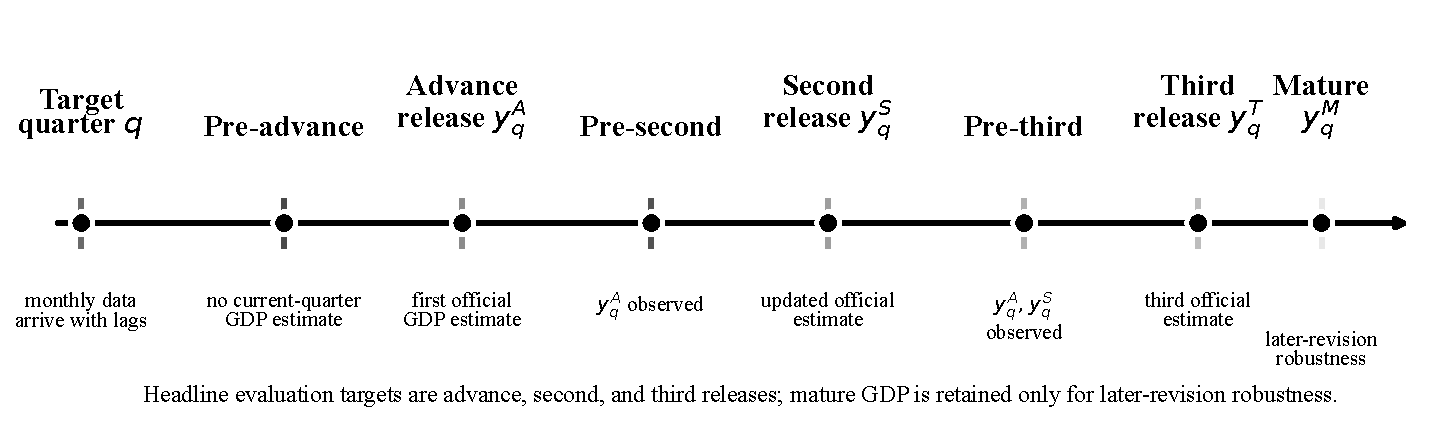
\includegraphics[width=1\textwidth]{figures/release_ladder_timeline.pdf}
\caption{GDP release ladder and forecast checkpoints.}
\label{fig:release_ladder_timeline}
\end{figure}

The release ladder is written as
\[
\mathbf y_q=(y_q^{\Arel},y_q^{\Srel},y_q^{\Trel},y_q^{\Mrel})',
\]
with adjacent revisions
\[
\dSA_q=y_q^{\Srel}-y_q^{\Arel},\qquad
\dTS_q=y_q^{\Trel}-y_q^{\Srel},\qquad
\dMT_q=y_q^{\Mrel}-y_q^{\Trel}.
\]
This notation separates the forecast target from the evaluation vintage. A pre-second forecast of $y_q^{\Srel}$ is not equivalent to a pre-advance forecast of $y_q^{\Arel}$, even though both refer to the same calendar quarter.

At a forecast origin $d$ where release $r_1$ is public and $r_2$ is the next release, squared-error optimality gives
\[
E_d[y_q^{r_2}]=y_q^{r_1}+E_d[y_q^{r_2}-y_q^{r_1}].
\]
Thus later-release nowcasting is a revision-forecasting problem: a model improves no-revision in point loss only by estimating a nonzero conditional mean revision, while density gains can arise from modelling revision variance and covariance.

\subsection{Information sets, timing, and leakage controls}

Exact timing uses only ALFRED vintages dated no later than the forecast origin, defined as one business day before the mapped GDP release date. For 2005Q1--2024Q4, all 240 A/S/T checkpoint dates are mapped from GDPC1 vintage-derived release dates. Pseudo timing is retained only as a robustness comparison with a coarser month-end cutoff. Current-quarter GDP releases are masked until public; monthly observations enter only if their vintage date is admissible; and SPF and no-revision rows appear only at compatible checkpoints. Table~\ref{tab:data_architecture} reports the component audit.

Formally, let $\mathcal I_{q,c}(d)$ denote the information set for quarter $q$ at checkpoint $c$ and origin date $d$. It contains only monthly observations, GDP releases, and survey forecasts admissible at $d$. Forecasts are functions of $\mathcal I_{q,c}(d)$ rather than of a final dataset, ruling out later monthly vintages and not-yet-public GDP estimates.

\begingroup
\small
\setlength{\tabcolsep}{3pt}
\setlength{\LTleft}{0pt}
\setlength{\LTright}{0pt}
\begin{longtable}{L{2.8cm}L{3.5cm}L{8.4cm}}
\caption{Data architecture and leakage controls}\label{tab:data_architecture}\\
\toprule
Component & Role & Leakage-control rule \\
\midrule
\endfirsthead
\toprule
Component & Role & Leakage-control rule \\
\midrule
\endhead
GDP release targets & Define $y_q^{\Arel}$, $y_q^{\Srel}$, $y_q^{\Trel}$, $y_q^{\Mrel}$ and adjacent revisions. & Current-quarter releases are masked until their public checkpoint; mature targets are robustness targets only. \\
Monthly indicators & Supply labour, production, income, spending, housing, trade, inventory, and rate information. & A monthly observation enters only if its vintage date is no later than the forecast origin. \\
GDP release calendar & Determines exact pre-release forecast origins for A/S/T targets. & Headline dates are GDPC1 vintage-date derived; fallback rows are separated from headline evidence. \\
SPF and no-revision & Provide the external pre-advance and institutional later-release benchmarks. & SPF must be timing-compatible; no-revision uses only an already public GDP estimate for the same quarter. \\
Evaluation design & Defines point, density, revision-risk, timing, and robustness checks. & Scores use only admissible real-time information and separate A/S/T evidence from mature robustness. \\
\bottomrule
\end{longtable}
\endgroup

Formally, the later-release no-revision rule is
\[
\widehat y_{q,\mathrm{pre\text{-}second}}^{\Srel}=y_q^{\Arel},\qquad
\widehat y_{q,\mathrm{pre\text{-}third}}^{\Trel}=y_q^{\Srel}.
\]
Before the advance release, no official current-quarter GDP estimate exists, so SPF is the relevant external point benchmark. After the advance release, no-revision is the institutional benchmark. The comparison is therefore deliberately demanding: models compete with professional judgment before the first release and with the latest official estimate after the first release.

This timing discipline is stricter than a calendar-quarter split because it determines which monthly observations, survey forecasts, and GDP estimates can be used at each checkpoint.

\subsection{Econometric framework and benchmark architecture}
\label{sec:model}

The empirical comparison uses five classes: SPF and no-revision benchmarks, AR/bridge/MIDAS regressions, dynamic-factor benchmarks, quarterly release-revision state-space models (SSMs), and a monthly mixed-frequency state-space robustness benchmark (MF-SSM). Table~\ref{tab:model_mapping} gives the detailed mapping. The headline state-space rows are quarterly release-ladder systems; monthly information is made vintage-correct and transformed into checkpoint-specific quarterly inputs.

\begingroup
\small
\setlength{\tabcolsep}{3pt}
\setlength{\LTleft}{0pt}
\setlength{\LTright}{0pt}
\begin{longtable}{L{2.9cm}L{3.5cm}L{8.4cm}}
\caption{Model and benchmark architecture}\label{tab:model_mapping}\\
\toprule
Label & Model class & Manuscript role \\
\midrule
\endfirsthead
\toprule
Label & Model class & Manuscript role \\
\midrule
\endhead
SPF & External professional forecast & Main pre-advance point benchmark. \\
No-revision & Institutional carry-forward rule & Main later-release point benchmark. \\
AR, bridge, MIDAS/UMIDAS & Low-dimensional and mixed-frequency regressions & Conventional statistical competitors. \\
Release DFM & Release-origin factor benchmark & Dynamic-factor comparator using checkpoint-specific quarterly inputs. \\
GDP-revision SSM & Quarterly release-revision state-space model & Main release-ladder state-space specification. \\
Indicator-revision SSM & Source-indicator revision extension & Tests whether indicator vintages add revision information. \\
Joint-revision SSM & GDP and indicator revision state-space model & Combines the two revision channels. \\
Monthly MF-SSM & Monthly mixed-frequency state-space benchmark & Secondary robustness benchmark with direct monthly observations. \\
\bottomrule
\end{longtable}
\endgroup

The state-space specification is deliberately low-dimensional: it isolates whether release-specific target alignment changes the benchmark hierarchy. The release-revision state captures systematic differences between early and later GDP estimates, while the quarterly activity component captures the common signal in the vintage-correct monthly panel.

Let $z_{q,c}$ denote the vector of vintage-correct monthly information aggregated into a release-origin-specific quarterly input at checkpoint $c$. The main state-space system contains a latent quarterly activity component $g_q$ and a release-revision component $s_q$. The transition block can be written generically as
\[
\alpha_q = F\alpha_{q-1}+u_q, \qquad u_q\sim N(0,Q),
\]
where $\alpha_q$ contains $g_q$, $s_q$, and any auxiliary factor dynamics. The quarterly input block is
\[
z_{q,c}=H_c\alpha_q+v_{q,c}, \qquad v_{q,c}\sim N(0,R_c),
\]
where the checkpoint-specific matrix $H_c$ reflects which vintage-correct monthly inputs are admissible at the forecast origin.

The GDP release block is
\begin{align}
 y_q^{\Arel} &= \mu_{\Arel}+g_q+s_q+\varepsilon_q^{\Arel}, \\
 y_q^{\Srel} &= \mu_{\Srel}+g_q+\psi_{\Srel}s_q+\varepsilon_q^{\Srel}, \\
 y_q^{\Trel} &= \mu_{\Trel}+g_q+\psi_{\Trel}s_q+\varepsilon_q^{\Trel}, \\
 y_q^{\Mrel} &= \mu_{\Mrel}+g_q+\varepsilon_q^{\Mrel},
\end{align}
with $0\leq \psi_{\Trel}\leq \psi_{\Srel}\leq 1$. The normalization gives the advance release full exposure to the release-revision state and gives the mature target zero exposure. The restrictions are statistical rather than structural: they summarize declining early-release exposure without claiming to identify every institutional source of GDP revision.

The loading restriction anchors the interpretation of $s_q$ and prevents an unrestricted latent factor from relabelling arbitrary release differences as revisions. This identification is sufficient for predictive means, variances, and release contrasts, but it is not a causal decomposition of BEA source-data revisions.

The Kalman filter produces predictive means and covariance matrices for the release vector. If $\mu_{q|d}$ and $\Sigma_{q|d}$ are the predictive mean and covariance for $(y_q^{\Arel},y_q^{\Srel},y_q^{\Trel},y_q^{\Mrel})'$ at origin $d$, adjacent-revision moments are
\begin{align}
\mathbb E_d[\Delta_q^{r_2,r_1}] &= e_{r_2}'\mu_{q|d}-e_{r_1}'\mu_{q|d}, \\
\mathbb V_d[\Delta_q^{r_2,r_1}] &= (e_{r_2}-e_{r_1})'\Sigma_{q|d}(e_{r_2}-e_{r_1}),
\end{align}
where $e_r$ selects release $r$. Indicator-revision and joint-revision variants add source-indicator revision states; the monthly MF-SSM uses direct monthly observation equations and sparse GDP observations. State-space rows use model-implied predictive variances when available, while non-state-space, SPF, and no-revision rows use expanding residual-calibrated Gaussian densities.

\subsection{Recursive forecast design and evaluation}
\label{sec:evaluation}

The baseline evaluates exact-vintage recursive forecasts over 2005Q1--2024Q4. The expanding-window design uses at least 48 training quarters, one factor, an EM cap of 100 iterations, and MIDAS lag length 6. The exact point sample contains 80 pre-advance forecasts, 79 pre-second forecasts, and 80 pre-third forecasts.

The recursive design re-estimates models, calibrates benchmarks, constructs residual-based densities, and runs numerical diagnostics using only information available up to each origin. Differences across checkpoints are therefore interpreted as differences in public information sets rather than artifacts of inconsistent estimation windows.

For a model $m$, checkpoint $c$, target $r$, and timing mode $\tau$, the point forecast error is
\[
e_{q,c,r,m}^{\tau}=\widehat y_{q,c,r,m}^{\tau}-y_q^r.
\]
Forecast errors are reported as forecast minus realized values, so bias is positive when forecasts exceed realizations on average. The main point scores are root mean squared error (RMSE) and mean absolute error (MAE):
\[
\mathrm{RMSE}_{c,r,m}=\left(N^{-1}\sum_q (e_{q,c,r,m}^{\tau})^2\right)^{1/2},\quad
\mathrm{MAE}_{c,r,m}=N^{-1}\sum_q |e_{q,c,r,m}^{\tau}|,
\]
with bias equal to the sample mean of $e_{q,c,r,m}^{\tau}$. Revision forecasts use the same scoring rules applied to adjacent revision targets $\dSA_q$, $\dTS_q$, and $\dMT_q$. Directional accuracy is reported only for models that issue nonzero positive or negative revision signals; a zero-revision forecast does not supply a directional classification and is therefore marked not applicable for raw sign accuracy.

Density metrics include log score, CRPS, interval coverage, predictive standard deviation, probability integral transform diagnostics, and a below-zero Brier score. For predictive distribution $F$ and realization $y$,
\[
\mathrm{CRPS}(F,y)=\int_{-\infty}^{\infty}\left(F(z)-\mathbf 1\{y\leq z\}\right)^2dz.
\]
Residual-calibrated densities require historical forecast errors, so density sample sizes can differ; rankings are interpreted conservatively. Diebold--Mariano tests use Newey--West/HAC variance estimates with lag $\lfloor n^{1/3}\rfloor$, and model-confidence-set-style diagnostics use 5,000 moving-block bootstrap replications with block length 4. The empirical claims combine point loss, density evidence, revision-risk evidence, and these conservative diagnostics.

\section{Results and discussion}
\label{sec:results}

\noindent\textbf{Research questions.} The empirical section answers three questions: (RQ1) which benchmark wins at each release checkpoint; (RQ2) whether release-revision state-space structure improves density or revision-risk assessment when point RMSE does not; and (RQ3) whether the rankings survive timing, maturity, subsample, tuning, and numerical checks. Table~\ref{tab:rq_map} maps the empirical subsections to these questions.

\begingroup
\small
\setlength{\tabcolsep}{4pt}
\setlength{\LTleft}{0pt}
\setlength{\LTright}{0pt}
\begin{longtable}{L{3.1cm}L{1.4cm}L{8.8cm}}
\caption{Research-question map for the empirical section}\label{tab:rq_map}\\
\toprule
Empirical subsection & RQ & Role in the argument \\
\midrule
\endfirsthead
\toprule
Empirical subsection & RQ & Role in the argument \\
\midrule
\endhead
Point forecasts & RQ1 & Identifies the stage-specific point benchmark: SPF before advance, no-revision before second and third. \\
Exact versus pseudo timing & RQ3 & Checks timing discipline and leakage sensitivity. \\
Density and revision-risk results & RQ2 & Locates state-space value beyond point RMSE. \\
Forecast-comparison inference & RQ3 & Disciplines interpretation of small loss gaps. \\
Institutional release mechanism & RQ1--RQ2 & Explains the point-density contrast. \\
Robustness diagnostics & RQ3 & Tests maturity, subsample, tuning, and numerical stability. \\
\bottomrule
\end{longtable}
\endgroup

Read together, the subsections show that the point benchmark is stage-dependent, state-space value is strongest for uncertainty and revisions, and the ranking is not a timing or numerical artifact.

\subsection{Point forecasts}
\label{subsec:point}

Table~\ref{tab:point_results} reports the exact-timing point RMSE, MAE, and bias evidence. Figure~\ref{fig:point_rmse} reports RMSE gaps relative to the release-stage winner for the main operational competitors. The benchmark changes across the release ladder. Before the advance release, SPF has the lowest RMSE. Before the second and third releases, no-revision has the lowest RMSE. Release-aware state-space models are competitive at later checkpoints, but they do not dominate no-revision in point loss.

\begingroup
\small
\setlength{\tabcolsep}{5pt}
\setlength{\LTleft}{\fill}
\setlength{\LTright}{\fill}

\begin{longtable}{llrrrr}
\caption{Headline exact-timing point forecast results}\label{tab:point_results}\\

\toprule
Checkpoint & Model & $N$ & RMSE & MAE & Bias \\
\midrule
\endfirsthead

\toprule
Checkpoint & Model & $N$ & RMSE & MAE & Bias \\
\midrule
\endhead

Pre-advance $\rightarrow y^{\Arel}$ & SPF & 80 & 2.225 & 1.338 & 0.032 \\
 & Release DFM & 80 & 3.066 & 1.626 & 0.561 \\
 & GDP-revision SSM & 80 & 3.383 & 1.823 & 0.109 \\
 & Indicator-revision SSM & 80 & 3.566 & 2.102 & 0.303 \\
 & Joint-revision SSM & 80 & 3.610 & 1.986 & 0.155 \\
 & Monthly MF-SSM & 80 & 3.725 & 1.981 & 0.130 \\
 & Bridge & 80 & 4.874 & 2.074 & -0.087 \\

\addlinespace
Pre-second $\rightarrow y^{\Srel}$ & No-revision & 79 & 0.570 & 0.400 & -0.066 \\
 & Indicator-revision SSM & 79 & 0.591 & 0.447 & -0.019 \\
 & Monthly MF-SSM & 79 & 0.595 & 0.413 & 0.039 \\
 & Joint-revision SSM & 79 & 0.632 & 0.474 & 0.066 \\
 & Release DFM & 79 & 0.691 & 0.442 & -0.008 \\
 & GDP-revision SSM & 79 & 0.695 & 0.465 & 0.064 \\
 & SPF & 79 & 2.337 & 1.448 & -0.033 \\

\addlinespace
Pre-third $\rightarrow y^{\Trel}$ & No-revision & 80 & 0.362 & 0.240 & -0.048 \\
 & Monthly MF-SSM & 80 & 0.369 & 0.260 & 0.001 \\
 & Indicator-revision SSM & 80 & 0.371 & 0.242 & -0.049 \\
 & Joint-revision SSM & 80 & 0.372 & 0.246 & -0.041 \\
 & GDP-revision SSM & 80 & 0.373 & 0.246 & -0.039 \\
 & Release DFM & 80 & 0.445 & 0.287 & -0.004 \\
 & SPF & 80 & 2.380 & 1.481 & -0.081 \\

\bottomrule
\multicolumn{6}{
p{\dimexpr\textwidth-2\tabcolsep\relax}
}{
\footnotesize Notes: Bias is forecast minus realized. The no-revision pre-advance row is omitted from the table because no official current-quarter GDP estimate is available before the advance release.
}

\end{longtable}

\endgroup

\begin{figure}[H]
\centering
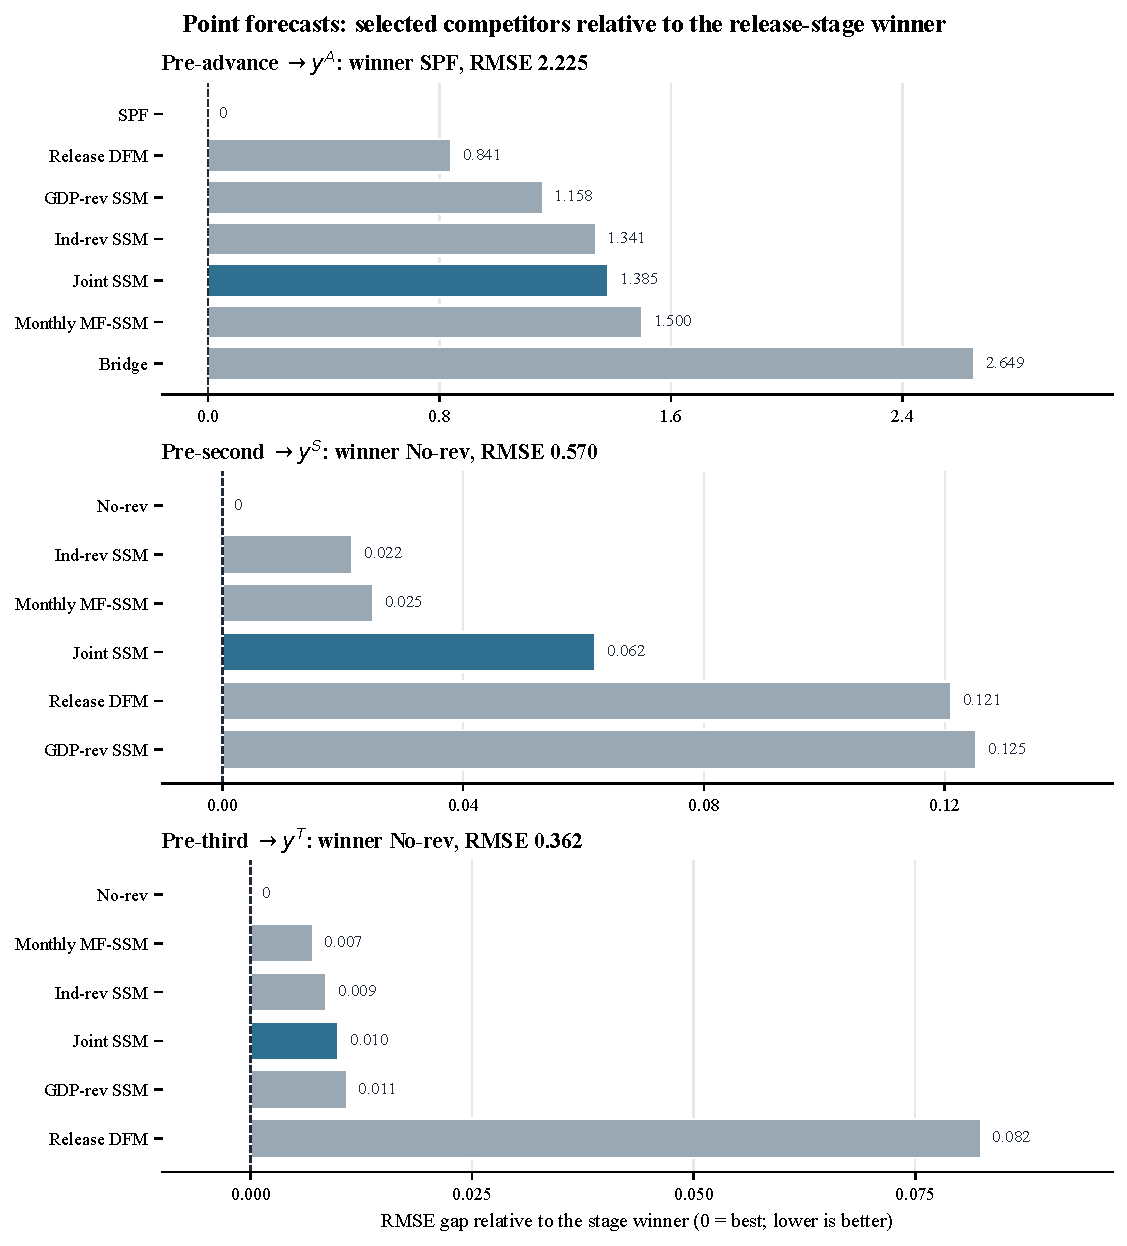
\includegraphics[width=1\textwidth]{figures/point_rmse_gap_to_benchmark.pdf}
\caption{Exact-timing point RMSE gaps relative to the release-stage winner.}
\label{fig:point_rmse}
\end{figure}

The interpretation is straightforward. Before the advance release, the model must nowcast the first official estimate and SPF performs best. Later checkpoints are different because an official estimate is already public; carrying it forward is a stringent benchmark. State-space rows narrow the gap relative to conventional bridge and DFM rows, but the headline point-loss result remains no-revision at the second and third checkpoints.

\subsection{Exact versus pseudo timing}
\label{subsec:exact_pseudo}

Exact and pseudo timing produce very similar conclusions. Table~\ref{tab:exact_pseudo_checks} shows that benchmark winners are unchanged, no-revision rows are identical by construction, and representative state-space gaps are small. Exact timing therefore supports leakage control rather than producing the ranking by a fragile dating convention.

\begingroup
\small
\setlength{\tabcolsep}{5pt}
\setlength{\LTleft}{\fill}
\setlength{\LTright}{\fill}
\begin{longtable}{L{2.5cm}L{3.7cm}rrr}
\caption{Exact-versus-pseudo timing checks}\label{tab:exact_pseudo_checks}\\
\toprule
Checkpoint & Model & Exact RMSE & Pseudo RMSE & Gap \\
\midrule
\endfirsthead
\toprule
Checkpoint & Model & Exact RMSE & Pseudo RMSE & Gap \\
\midrule
\endhead
Pre-advance & SPF & 2.225 & 2.225 & 0.000 \\
Pre-advance & Release DFM & 3.066 & 3.052 & 0.014 \\
Pre-advance & GDP-revision SSM & 3.383 & 3.380 & 0.003 \\
Pre-second & No-revision & 0.570 & 0.570 & 0.000 \\
Pre-second & Monthly MF-SSM & 0.595 & 0.593 & 0.001 \\
Pre-third & No-revision & 0.362 & 0.362 & 0.000 \\
Pre-third & Monthly MF-SSM & 0.369 & 0.369 & 0.000 \\
\bottomrule
\multicolumn{5}{p{\dimexpr\textwidth-2\tabcolsep\relax}}{\footnotesize Notes: Gap is exact minus pseudo RMSE. Rows are selected to show the headline benchmark and representative release-aware competitors.}
\end{longtable}
\endgroup

\subsection{Density forecasts}
\label{subsec:density}

Density scoring reveals a different part of the contribution. Table~\ref{tab:density_results} reports CRPS, effective sample size, and interval coverage, while Figure~\ref{fig:density_crps} reports CRPS gaps relative to the stage benchmark. The pre-advance density benchmark remains SPF, and before the second release no-revision remains strong. Before the third release, state-space rows cross below the no-revision benchmark, with the indicator-revision SSM slightly ahead of joint and GDP-revision variants. The interpretation is deliberately conservative: point-loss dominance is not claimed from density evidence, and density wins with different $N$ are read as evidence about uncertainty quantification rather than as unconditional model superiority.

\begingroup
\small
\setlength{\tabcolsep}{5pt}
\setlength{\LTleft}{\fill}
\setlength{\LTright}{\fill}

\begin{longtable}{lllrrr}
\caption{Headline exact-timing density and revision-risk results}\label{tab:density_results}\\

\toprule
Panel & Target & Model & $N$ & CRPS & 90\% coverage \\
\midrule
\endfirsthead

\toprule
Panel & Target & Model & $N$ & CRPS & 90\% coverage \\
\midrule
\endhead

Point density & $y^{\Arel}$ & SPF & 68 & 1.066 & 0.897 \\
 & $y^{\Arel}$ & Release DFM & 68 & 1.371 & 0.853 \\
 & $y^{\Arel}$ & GDP-revision SSM & 80 & 1.435 & 0.875 \\

\addlinespace
 & $y^{\Srel}$ & No-revision & 67 & 0.300 & 0.940 \\
 & $y^{\Srel}$ & Monthly MF-SSM & 79 & 0.316 & 0.911 \\
 & $y^{\Srel}$ & Indicator-revision SSM & 79 & 0.326 & 0.911 \\

\addlinespace
 & $y^{\Trel}$ & Indicator-revision SSM & 80 & 0.187 & 0.938 \\
 & $y^{\Trel}$ & Joint-revision SSM & 80 & 0.188 & 0.938 \\
 & $y^{\Trel}$ & GDP-revision SSM & 80 & 0.188 & 0.938 \\
 & $y^{\Trel}$ & No-revision & 68 & 0.198 & 0.868 \\

\midrule
Revision density & $\dSA$ & No-revision & 67 & 0.300 & 0.940 \\
 & $\dSA$ & Indicator-revision SSM & 79 & 0.308 & 0.937 \\
 & $\dSA$ & Monthly MF-SSM & 79 & 0.327 & 0.911 \\

\addlinespace
 & $\dTS$ & GDP-revision SSM & 79 & 0.184 & 0.949 \\
 & $\dTS$ & Joint-revision SSM & 79 & 0.184 & 0.949 \\
 & $\dTS$ & Indicator-revision SSM & 79 & 0.184 & 0.949 \\
 & $\dTS$ & No-revision & 67 & 0.197 & 0.866 \\

\addlinespace
 & $\dMT$ & No-revision & 68 & 0.752 & 0.897 \\
 & $\dMT$ & Release DFM & 68 & 0.760 & 0.882 \\
 & $\dMT$ & Indicator-revision SSM & 80 & 0.803 & 0.975 \\

\bottomrule
\multicolumn{6}{
p{\dimexpr\textwidth-2\tabcolsep\relax}
}{
\footnotesize Notes: CRPS is lower-is-better. Each row reports its effective density-evaluation sample. Residual-calibrated benchmark densities require a calibration window, while state-space rows can use model-implied predictive covariance. For this reason, density rankings are interpreted conservatively and are not used to claim universal point-forecast dominance. $\dMT$ is mature-target robustness, not a headline point target.
}

\end{longtable}

\endgroup

\begin{figure}[H]
\centering
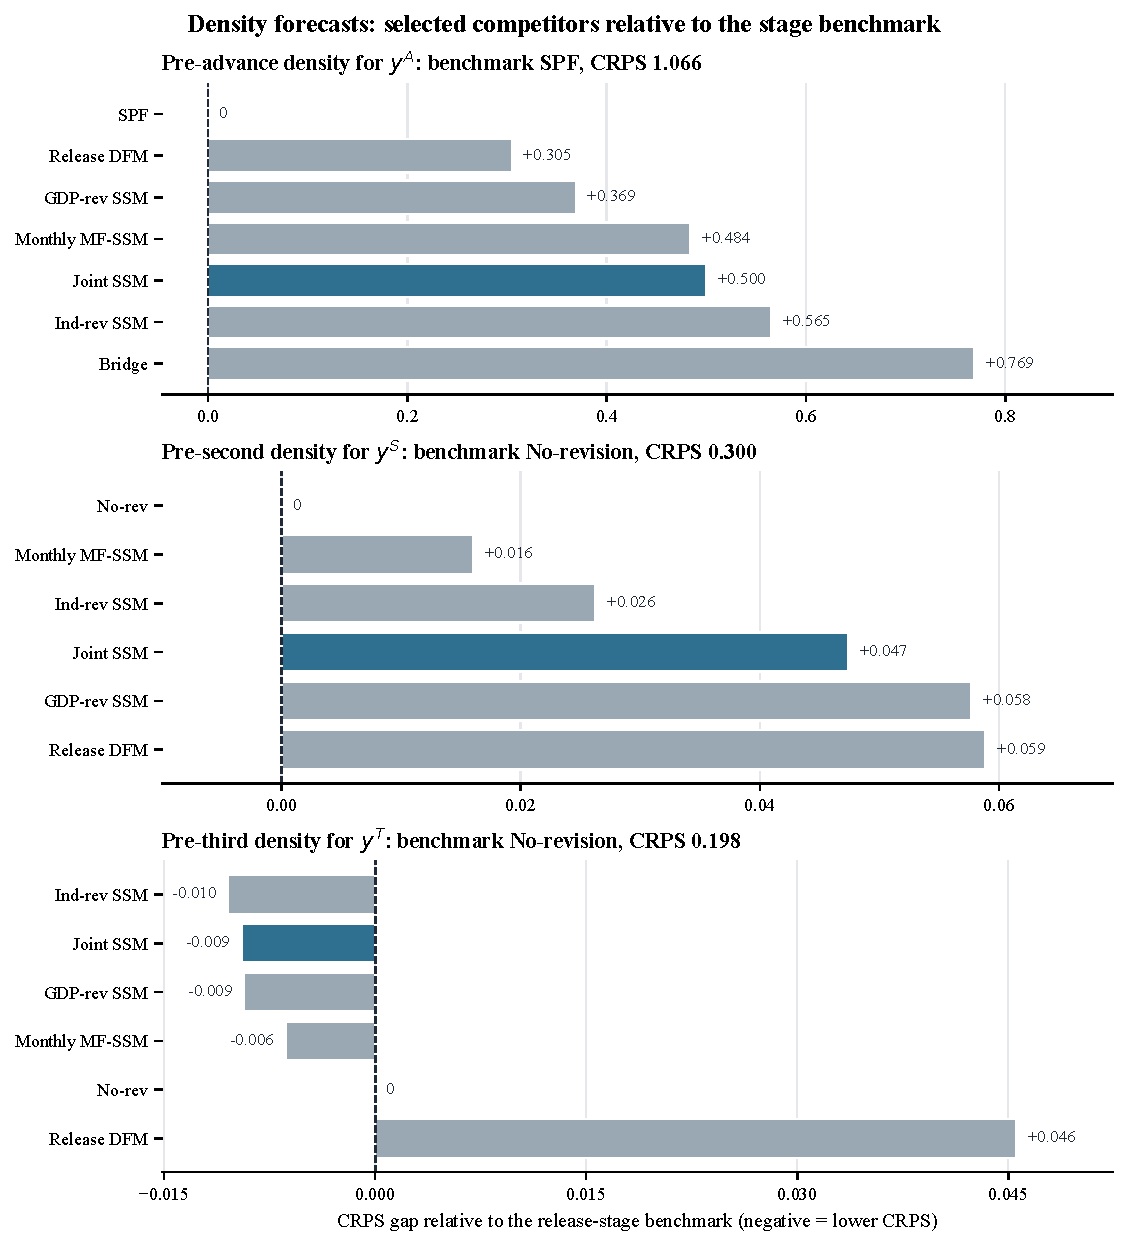
\includegraphics[width=1\textwidth]{figures/density_crps_gap_to_benchmark.pdf}
\caption{Point-density CRPS gaps relative to the release-stage benchmark.}
\label{fig:density_crps}
\end{figure}

The density evidence supports a narrower claim than point dominance. Release-aware covariance structure helps quantify uncertainty in later-release targets and adjacent revisions. The third-release result is the clearest case: the model-implied covariance matrix links successive GDP releases, so the same system can produce a predictive distribution for both the next release and the adjacent revision.


\subsection{Revision forecasts and revision-risk densities}
\label{subsec:revision}

Adjacent revisions matter because users may care about the likelihood and size of changes between official estimates. Table~\ref{tab:revision_summary} combines the point and density evidence. Point forecasts of revisions are hard to improve upon because zero or near-zero revisions are strong RMSE benchmarks. The main distributional gain appears for $\dTS$, where release-aware state-space rows have CRPS near 0.184 compared with 0.197 for no-revision, as also shown in Table~\ref{tab:density_results}.

The $\dMT$ rows are retained because mature revisions are relevant for longer-run data reliability, but they do not redefine the headline nowcasting result. The main A/S/T evidence concerns the next official release. Figure~\ref{fig:revision_crps} visualizes the adjacent-revision CRPS gaps relative to no-revision.

\begingroup
\small
\setlength{\tabcolsep}{4pt}
\setlength{\LTleft}{\fill}
\setlength{\LTright}{\fill}
\begin{longtable}{L{2.0cm}L{3.2cm}C{2.0cm}L{3.2cm}C{1.6cm}}
\caption{Adjacent-revision point and density summary}\label{tab:revision_summary}\\
\toprule
Target & Best point row & Point RMSE & Best density row & CRPS \\
\midrule
\endfirsthead
\toprule
Target & Best point row & Point RMSE & Best density row & CRPS \\
\midrule
\endhead
$\dSA$ & No-revision tie & 0.570 & No-revision & 0.300 \\
$\dTS$ & No-revision tie & 0.361 & SSM tie & 0.184 \\
$\dMT$ & No-revision tie & 1.339 & No-revision & 0.752 \\
\bottomrule
\multicolumn{5}{p{\dimexpr\textwidth-2\tabcolsep\relax}}{\footnotesize Notes: Point ties include SPF and indicator-revision SSM rows where the reported zero-revision forecast has the same rounded RMSE. The SSM density tie for $\dTS$ includes GDP-revision, joint-revision, and indicator-revision state-space rows.}
\end{longtable}
\endgroup

\begin{figure}[H]
\centering
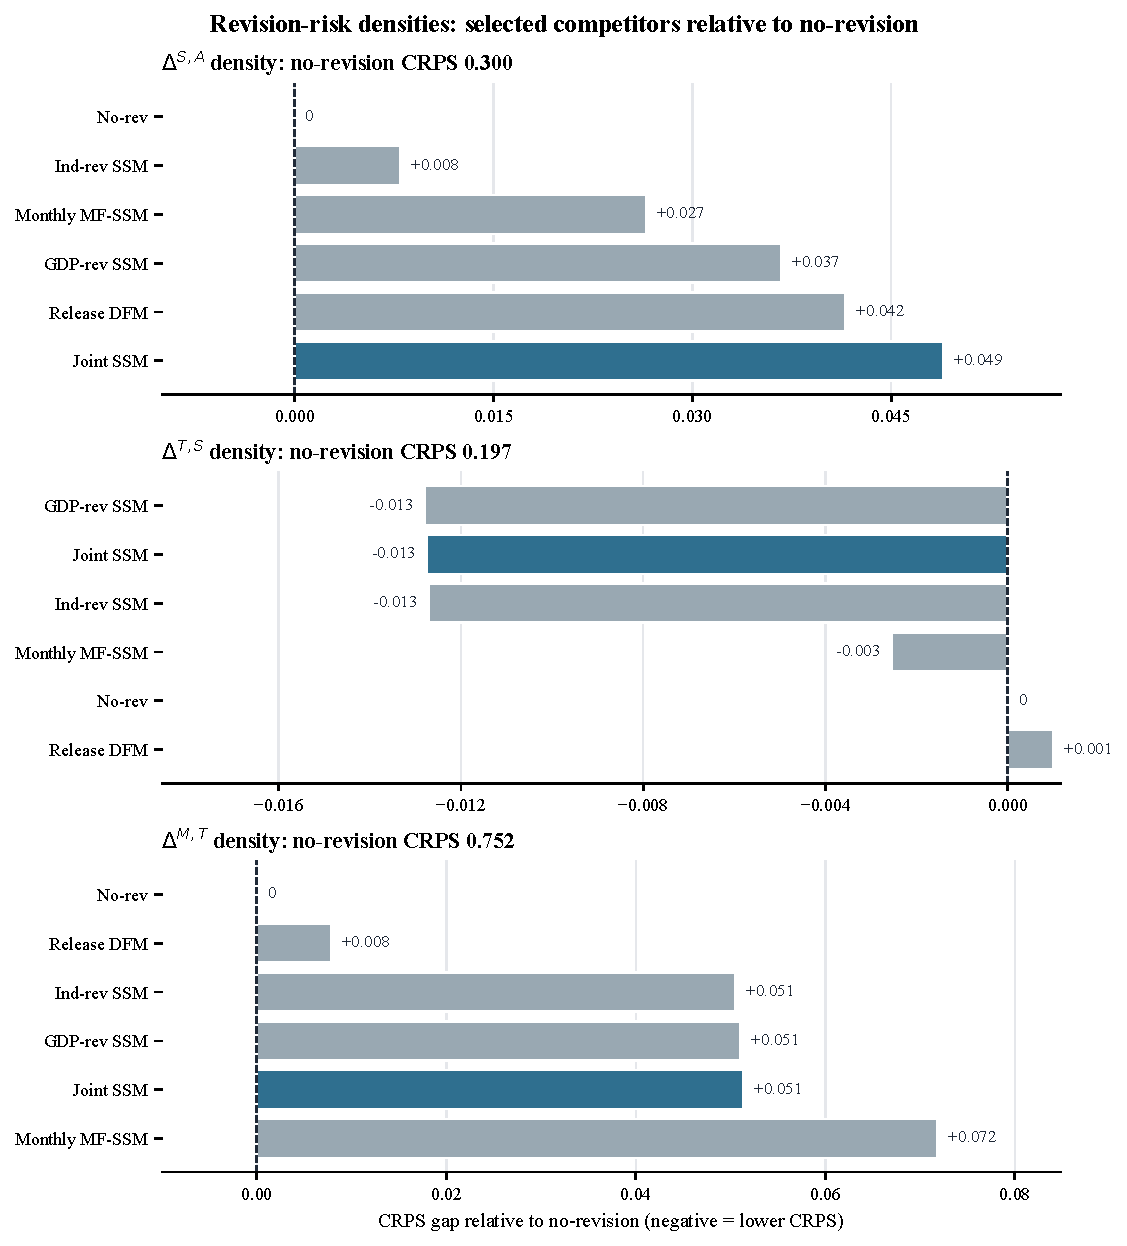
\includegraphics[width=1\textwidth]{figures/revision_density_crps_gap_to_no_revision.pdf}
\caption{Adjacent-revision density CRPS gaps relative to no-revision.}
\label{fig:revision_crps}
\end{figure}

\subsection{Forecast-comparison inference}
\label{subsec:inference}

The inference diagnostics support a conservative reading. Table~\ref{tab:inference_summary} reports model-confidence-set-style block-bootstrap results. At the 10 percent elimination threshold, most models remain in the final set for later-release point forecasts, consistent with the small RMSE differences in Table~\ref{tab:point_results}. For revision targets, final sets are smaller but still include several competing rows. The inference therefore identifies benchmark difficulty and the economic role of official releases, not a statistically isolated universal champion model.

\begingroup
\small
\setlength{\tabcolsep}{3pt}
\begin{longtable}{L{1.8cm}C{1.5cm}C{1.3cm}C{1.3cm}C{0.9cm}C{1.1cm}L{4.8cm}}
\caption{Forecast-comparison inference summary}\label{tab:inference_summary}\\
\toprule
Family & Target & Initial & Final & $N$ & Reps & Main interpretation \\
\midrule
\endfirsthead
\toprule
Family & Target & Initial & Final & $N$ & Reps & Main interpretation \\
\midrule
\endhead
Point & $y^{\Arel}$ & 11 & 10 & 80 & 5000 & SPF leads; only MIDAS/UMIDAS is eliminated. \\
Point & $y^{\Srel}$ & 11 & 11 & 79 & 5000 & Later-release point gaps are not decisive. \\
Point & $y^{\Trel}$ & 11 & 11 & 80 & 5000 & No-revision leads, but gaps are small. \\
Revision & $\dSA$ & 11 & 10 & 79 & 5000 & Zero/no-revision remains competitive. \\
Revision & $\dTS$ & 11 & 9 & 79 & 5000 & State-space density evidence is stronger than point ranking. \\
Revision & $\dMT$ & 11 & 8 & 80 & 5000 & Mature-revision robustness, not headline A/S/T evidence. \\
\bottomrule
\multicolumn{7}{p{\dimexpr\textwidth-2\tabcolsep\relax}}{\footnotesize Notes: The block length is 4 and the nominal elimination level is 10 percent. These diagnostics are used to avoid overinterpreting small loss gaps.}
\end{longtable}
\endgroup

For applied use, the evidence rejects universal point-loss dominance by release-aware state-space models, but supports their role in uncertainty assessment. Given the sample size and small later-release gaps, it does not justify a universal model-ranking claim.



\subsection{Institutional release mechanism}
\label{subsec:mechanism}

The mechanism behind the headline result is institutional. Once the advance or second estimate is public, it is an official aggregate of source data, survey data, and BEA methods. That estimate is difficult to improve upon in point loss using the remaining monthly indicators before the next release. Release-aware state-space models are still useful because they quantify covariance across releases and uncertainty around revisions.


\subsection{Robustness, sensitivity, and numerical diagnostics}
\label{sec:robustness}

Robustness evidence checks whether the release-ladder conclusions depend on maturity conventions, sample segmentation, tuning choices, or numerical failures. Table~\ref{tab:robustness_diagnostics} reports the checks. The baseline remains the non-mature A/S/T evaluation; mature-target variants test later-revision sensitivity only.

\begingroup
\footnotesize
\setlength{\tabcolsep}{3pt}
\setlength{\LTleft}{0pt}
\setlength{\LTright}{0pt}
\begin{longtable}{L{2.3cm}L{4.5cm}rrL{4.2cm}}
\caption{Quantitative robustness, sensitivity, and numerical diagnostics}\label{tab:robustness_diagnostics}\\
\toprule
Block & Statistic & Baseline & Check & Difference or diagnostic \\
\midrule
\endfirsthead
\toprule
Block & Statistic & Baseline & Check & Difference or diagnostic \\
\midrule
\endhead
Timing & Release DFM pre-advance RMSE & 3.066 & 3.052 & Exact minus pseudo $=0.014$. \\
Timing & GDP-revision SSM pre-advance RMSE & 3.383 & 3.380 & Exact minus pseudo $=0.003$. \\
Timing & Monthly MF-SSM pre-third RMSE & 0.369 & 0.369 & Exact minus pseudo rounds to 0.000. \\
\addlinespace
Mature target & $\dMT$ RMSE, one-year maturity & 1.339 & 1.002 & Lower by 0.337; A/S/T point winners unchanged. \\
Mature target & $\dMT$ RMSE, three-year maturity & 1.339 & 1.419 & Higher by 0.080; A/S/T point winners unchanged. \\
Mature target & $\dMT$ RMSE, latest maturity & 1.339 & 1.339 & Essentially unchanged; A/S/T point winners unchanged. \\
\addlinespace
Subsample & Pre-advance winner RMSE & 2.225 & 1.619 & SPF remains the winner when pandemic quarters are excluded. \\
Subsample & Pre-second winner RMSE & 0.570 & 0.557 & Winner shifts narrowly from no-revision to Monthly MF-SSM. \\
Subsample & Pre-third winner RMSE & 0.362 & 0.363 & No-revision remains the winner. \\
\addlinespace
Sensitivity grid & Exact A/S/T winner cells tested & 30 & 30 & All cells preserve the headline winners across 10 robustness builds. \\
Numerics & State-space convergence rate, exact rows & 1.000 & 1.000 & Min and max convergence rates are both 1.000. \\
Numerics & State-space covariance PSD share, exact rows & 1.000 & 1.000 & Min and max PSD shares are both 1.000. \\
\bottomrule
\multicolumn{5}{p{\dimexpr\textwidth-2\tabcolsep\relax}}{\footnotesize Notes: Baseline is the exact-timing non-mature run unless otherwise stated. The check column reports the pseudo-timing, mature-target, exclude-pandemic, sensitivity-grid, or numerical-audit value. $\dMT$ is mature-target robustness rather than a headline A/S/T point target.}
\end{longtable}
\endgroup

The robustness table shows that exact-vintage alignment is a leakage safeguard, mature-revision evidence is more variable than the A/S/T headline exercise, and the broad benchmark hierarchy is stable except for a narrow pre-second non-pandemic cell. These diagnostics support the density evidence but do not convert selected density wins into universal point-forecast dominance.

\subsection{Why release structure matters}
\label{sec:discussion}

Release structure matters because it changes both the loss comparison and the economic question. A pre-advance nowcast predicts the first official estimate; a pre-second forecast predicts how the advance estimate will be modified; and a pre-third forecast predicts how the second estimate will change. These are distinct objects, and the strongest benchmark changes accordingly.

This perspective also explains why density forecasting remains valuable when point RMSE does not improve. Users may need probabilities, intervals, and revision-risk measures around the latest official estimate. A single headline nowcast can hide whether the forecast predicts the first published estimate, updates an already published estimate, or describes revision risk.

Overall, Section~\ref{sec:results} answers RQ1 through the stage-specific benchmark hierarchy, RQ2 through density and revision-risk gains from release-aware covariance modelling, and RQ3 through timing, inference, robustness, and numerical checks.


\section{Conclusion and limitations}
\label{sec:conclusion_limitations}

The results support a release-ladder interpretation of GDP nowcasting, but the evidence should be read with appropriate scope conditions.

\subsection{Scope conditions and threats to validity}
\label{sec:limitations}

Several limitations should guide interpretation. First, the evaluation sample contains about 80 quarters, so forecast-comparison inference has limited power and large events can affect RMSE. Second, SPF is an external professional benchmark but does not directly target BEA release rounds in the same way the constructed A/S/T targets do. Third, the release-revision state is statistical rather than structural. Fourth, density variance construction differs across model classes: state-space rows use model-implied predictive covariance when available, whereas non-state-space benchmarks use residual-calibrated Gaussian densities. Fifth, the aggregate GDP system does not impose expenditure-side accounting identities. Sixth, exact timing is daily rather than intraday. Seventh, mature revisions may reflect methodological, annual, and benchmark revisions not captured by monthly indicators near the original release date.

These limitations motivate conservative language. The article does not claim that release-aware Kalman/EM models dominate all benchmarks. It claims that release-ladder evaluation changes the benchmark hierarchy and reveals distributional revision-risk value that point RMSE alone can miss.

Future work could add a larger indicator panel, expenditure-side constraints, survey nowcasts beyond SPF, and intraday release calendars, while retaining the release-stage benchmark hierarchy.


\subsection{Conclusion}
\label{sec:conclusion}

This article studies US real GDP nowcasting as a release-ladder problem. The operational target depends on the public release stage: advance before the first official release, second before the second release, third before the third release, and mature only for later-revision robustness. The empirical design aligns targets, forecast origins, and real-time information sets, then evaluates professional, institutional, conventional, and state-space benchmarks.

The main empirical result is release-stage dependence. SPF is the strongest pre-advance point benchmark. Once an official GDP estimate is public, no-revision is hard to beat before the second and third releases. Release-aware state-space models are competitive but do not provide universal point-RMSE dominance. Their clearest contribution is to density forecasts, predictive intervals, and adjacent revision-risk diagnostics.

This finding clarifies where the model-based contribution lies. Before the first release, the key task is extracting current-quarter information from monthly indicators and professional expectations. After the first release, the key task is assessing revision risk around a strong official benchmark.

For applied nowcasting, the implication is simple: the benchmark must match the release stage. Treating GDP nowcasting as a single final-vintage prediction exercise can obscure the institutional information already available to forecasters and can overstate the gains from statistical models. A release-ladder design gives a more credible and operationally relevant assessment of what nowcasting models can and cannot add.

The practical recommendation is therefore to report forecasts by checkpoint. Before the first official estimate, professional forecast comparisons remain central. After the advance estimate is public, any model should report both its point gain relative to no-revision and its revision-risk distribution.


\begin{thebibliography}{99}

\bibitem[Aastveit et al.(2014)]{aastveit2014}
Aastveit, K. A., Gerdrup, K. R., Jore, A. S., and Thorsrud, L. A. (2014).
Nowcasting GDP in real time: A density combination approach.
\emph{Journal of Business and Economic Statistics}, 32(1), 48--68. doi:\href{https://doi.org/10.1080/07350015.2013.844155}{10.1080/07350015.2013.844155}.

\bibitem[Anesti et al.(2022)]{anesti2022}
Anesti, N., Galvao, A. B., and Miranda-Agrippino, S. (2022).
Uncertain Kingdom: Nowcasting GDP and its revisions.
\emph{Journal of Applied Econometrics}, 37(1), 42--62. doi:\href{https://doi.org/10.1002/jae.2845}{10.1002/jae.2845}.

\bibitem[Bai and Ng(2002)]{bai2002}
Bai, J. and Ng, S. (2002).
Determining the number of factors in approximate factor models.
\emph{Econometrica}, 70(1), 191--221. doi:\href{https://doi.org/10.1111/1468-0262.00273}{10.1111/1468-0262.00273}.

\bibitem[Banbura and Modugno(2014)]{banburamodugno2014}
Banbura, M. and Modugno, M. (2014).
Maximum likelihood estimation of factor models on datasets with arbitrary pattern of missing data.
\emph{Journal of Applied Econometrics}, 29(1), 133--160. doi:\href{https://doi.org/10.1002/jae.2306}{10.1002/jae.2306}.

\bibitem[Banbura et al.(2013)]{banbura2013}
Banbura, M., Giannone, D., Modugno, M., and Reichlin, L. (2013).
Now-casting and the real-time data flow.
In G. Elliott and A. Timmermann (Eds.), \emph{Handbook of Economic Forecasting}, Vol. 2A, 195--237. Elsevier. doi:\href{https://doi.org/10.1016/B978-0-444-53683-9.00004-9}{10.1016/B978-0-444-53683-9.00004-9}.

\bibitem[Bok et al.(2018)]{bok2018}
Bok, B., Caratelli, D., Giannone, D., Sbordone, A. M., and Tambalotti, A. (2018).
Macroeconomic nowcasting and forecasting with big data.
\emph{Annual Review of Economics}, 10, 615--643. doi:\href{https://doi.org/10.1146/annurev-economics-080217-053214}{10.1146/annurev-economics-080217-053214}.

\bibitem[Clark and West(2007)]{clarkwest2007}
Clark, T. E. and West, K. D. (2007).
Approximately normal tests for equal predictive accuracy in nested models.
\emph{Journal of Econometrics}, 138(1), 291--311. doi:\href{https://doi.org/10.1016/j.jeconom.2006.05.023}{10.1016/j.jeconom.2006.05.023}.

\bibitem[Clements and Galvao(2008)]{clementsgalvao2008}
Clements, M. P. and Galvao, A. B. (2008).
Macroeconomic forecasting with mixed-frequency data.
\emph{Journal of Business and Economic Statistics}, 26(4), 546--554. doi:\href{https://doi.org/10.1198/073500108000000015}{10.1198/073500108000000015}.

\bibitem[Clements and Galvao(2013a)]{clementsgalvao2012}
Clements, M. P. and Galvao, A. B. (2013a).
Forecasting with vector autoregressive models of data vintages: US output growth and inflation.
\emph{International Journal of Forecasting}, 29(4), 698--714. doi:\href{https://doi.org/10.1016/j.ijforecast.2011.09.003}{10.1016/j.ijforecast.2011.09.003}.

\bibitem[Clements and Galvao(2013b)]{clementsgalvao2013}
Clements, M. P. and Galvao, A. B. (2013b).
Real-time forecasting of inflation and output growth with autoregressive models in the presence of data revisions.
\emph{Journal of Applied Econometrics}, 28(3), 458--477. doi:\href{https://doi.org/10.1002/jae.2274}{10.1002/jae.2274}.

\bibitem[Croushore and Stark(2001)]{croushorestark2001}
Croushore, D. and Stark, T. (2001).
A real-time data set for macroeconomists.
\emph{Journal of Econometrics}, 105(1), 111--130. doi:\href{https://doi.org/10.1016/S0304-4076(01)00072-0}{10.1016/S0304-4076(01)00072-0}.

\bibitem[Croushore and Stark(2003)]{croushorestark2003}
Croushore, D. and Stark, T. (2003).
A real-time data set for macroeconomists: Does the data vintage matter?
\emph{Review of Economics and Statistics}, 85(3), 605--617. doi:\href{https://doi.org/10.1162/003465303322369759}{10.1162/003465303322369759}.

\bibitem[Croushore(2011)]{croushore2011}
Croushore, D. (2011).
Frontiers of real-time data analysis.
\emph{Journal of Economic Literature}, 49(1), 72--100. doi:\href{https://doi.org/10.1257/jel.49.1.72}{10.1257/jel.49.1.72}.

\bibitem[Diebold and Mariano(1995)]{dieboldmariano1995}
Diebold, F. X. and Mariano, R. S. (1995).
Comparing predictive accuracy.
\emph{Journal of Business and Economic Statistics}, 13(3), 253--263. doi:\href{https://doi.org/10.1080/07350015.1995.10524599}{10.1080/07350015.1995.10524599}.

\bibitem[Doz et al.(2011)]{doz2011}
Doz, C., Giannone, D., and Reichlin, L. (2011).
A two-step estimator for large approximate dynamic factor models based on Kalman filtering.
\emph{Journal of Econometrics}, 164(1), 188--205. doi:\href{https://doi.org/10.1016/j.jeconom.2011.02.012}{10.1016/j.jeconom.2011.02.012}.

\bibitem[Doz et al.(2012)]{doz2012}
Doz, C., Giannone, D., and Reichlin, L. (2012).
A quasi-maximum likelihood approach for large, approximate dynamic factor models.
\emph{Review of Economics and Statistics}, 94(4), 1014--1024. doi:\href{https://doi.org/10.1162/REST_a_00225}{10.1162/REST\_a\_00225}.

\bibitem[Federal Reserve Bank of Philadelphia(2026a)]{philadelphiaRTDSM2026}
Federal Reserve Bank of Philadelphia (2026a).
Real-Time Data Set for Macroeconomists.
\url{https://www.philadelphiafed.org/surveys-and-data/real-time-data-research/real-time-data-set-for-macroeconomists}. Accessed 22 May 2026.

\bibitem[Federal Reserve Bank of Philadelphia(2026b)]{spf2026}
Federal Reserve Bank of Philadelphia (2026b).
Survey of Professional Forecasters.
\url{https://www.philadelphiafed.org/surveys-and-data/real-time-data-research/survey-of-professional-forecasters}. Accessed 22 May 2026.

\bibitem[Federal Reserve Bank of St. Louis(2026a)]{fred2026}
Federal Reserve Bank of St. Louis (2026a).
FRED Economic Data.
\url{https://fred.stlouisfed.org/}. Accessed 22 May 2026.

\bibitem[Federal Reserve Bank of St. Louis(2026b)]{alfred2026}
Federal Reserve Bank of St. Louis (2026b).
ALFRED: Archival Federal Reserve Economic Data.
\url{https://alfred.stlouisfed.org/}. Accessed 22 May 2026.

\bibitem[Forni et al.(2000)]{forni2000}
Forni, M., Hallin, M., Lippi, M., and Reichlin, L. (2000).
The generalized dynamic-factor model: Identification and estimation.
\emph{Review of Economics and Statistics}, 82(4), 540--554. doi:\href{https://doi.org/10.1162/003465300559037}{10.1162/003465300559037}.

\bibitem[Foroni et al.(2015)]{foroni2015}
Foroni, C., Marcellino, M., and Schumacher, C. (2015).
Unrestricted mixed data sampling (MIDAS): MIDAS regressions with unrestricted lag polynomials.
\emph{Journal of the Royal Statistical Society: Series A}, 178(1), 57--82. doi:\href{https://doi.org/10.1111/rssa.12043}{10.1111/rssa.12043}.

\bibitem[Ghysels et al.(2007)]{ghysels2007}
Ghysels, E., Sinko, A., and Valkanov, R. (2007).
MIDAS regressions: Further results and new directions.
\emph{Econometric Reviews}, 26(1), 53--90. doi:\href{https://doi.org/10.1080/07474930600972467}{10.1080/07474930600972467}.

\bibitem[Giacomini and Rossi(2010)]{giacominirossi2010}
Giacomini, R. and Rossi, B. (2010).
Forecast comparisons in unstable environments.
\emph{Journal of Applied Econometrics}, 25(4), 595--620. doi:\href{https://doi.org/10.1002/jae.1177}{10.1002/jae.1177}.

\bibitem[Giacomini and White(2006)]{giacominiwhite2006}
Giacomini, R. and White, H. (2006).
Tests of conditional predictive ability.
\emph{Econometrica}, 74(6), 1545--1578. doi:\href{https://doi.org/10.1111/j.1468-0262.2006.00718.x}{10.1111/j.1468-0262.2006.00718.x}.

\bibitem[Giannone et al.(2008)]{giannone2008}
Giannone, D., Reichlin, L., and Small, D. (2008).
Nowcasting: The real-time informational content of macroeconomic data.
\emph{Journal of Monetary Economics}, 55(4), 665--676. doi:\href{https://doi.org/10.1016/j.jmoneco.2008.05.010}{10.1016/j.jmoneco.2008.05.010}.

\bibitem[Gneiting and Raftery(2007)]{gneitingraftery2007}
Gneiting, T. and Raftery, A. E. (2007).
Strictly proper scoring rules, prediction, and estimation.
\emph{Journal of the American Statistical Association}, 102(477), 359--378. doi:\href{https://doi.org/10.1198/016214506000001437}{10.1198/016214506000001437}.

\bibitem[Gneiting et al.(2007)]{gneiting2007}
Gneiting, T., Balabdaoui, F., and Raftery, A. E. (2007).
Probabilistic forecasts, calibration and sharpness.
\emph{Journal of the Royal Statistical Society: Series B}, 69(2), 243--268. doi:\href{https://doi.org/10.1111/j.1467-9868.2007.00587.x}{10.1111/j.1467-9868.2007.00587.x}.

\bibitem[Hansen et al.(2011)]{hansen2011}
Hansen, P. R., Lunde, A., and Nason, J. M. (2011).
The model confidence set.
\emph{Econometrica}, 79(2), 453--497. doi:\href{https://doi.org/10.3982/ECTA5771}{10.3982/ECTA5771}.

\bibitem[Jacobs and van Norden(2011)]{jacobsvannorden2011}
Jacobs, J. P. A. M. and van Norden, S. (2011).
Modelling data revisions: Measurement error and dynamics of true values.
\emph{Journal of Econometrics}, 161(2), 101--109. doi:\href{https://doi.org/10.1016/j.jeconom.2010.04.010}{10.1016/j.jeconom.2010.04.010}.

\bibitem[Kishor and Koenig(2012)]{kishorkoenig2012}
Kishor, N. K. and Koenig, E. F. (2012).
VAR estimation and forecasting when data are subject to revision.
\emph{Journal of Business and Economic Statistics}, 30(2), 181--195. doi:\href{https://doi.org/10.1198/jbes.2010.08169}{10.1198/jbes.2010.08169}.

\bibitem[Koenig et al.(2003)]{koenig2003}
Koenig, E. F., Dolmas, S., and Piger, J. (2003).
The use and abuse of real-time data in economic forecasting.
\emph{Review of Economics and Statistics}, 85(3), 618--628. doi:\href{https://doi.org/10.1162/003465303322369768}{10.1162/003465303322369768}.

\bibitem[Kuzin et al.(2011)]{kuzin2011}
Kuzin, V., Marcellino, M., and Schumacher, C. (2011).
MIDAS versus mixed-frequency VAR: Nowcasting GDP in the euro area.
\emph{International Journal of Forecasting}, 27(2), 529--542. doi:\href{https://doi.org/10.1016/j.ijforecast.2010.02.006}{10.1016/j.ijforecast.2010.02.006}.

\bibitem[Landefeld et al.(2008)]{landefeld2008}
Landefeld, J. S., Seskin, E. P., and Fraumeni, B. M. (2008).
Taking the pulse of the economy: Measuring GDP.
\emph{Journal of Economic Perspectives}, 22(2), 193--216. doi:\href{https://doi.org/10.1257/jep.22.2.193}{10.1257/jep.22.2.193}.

\bibitem[Mankiw and Shapiro(1986)]{mankiwshapiro1986}
Mankiw, N. G. and Shapiro, M. D. (1986).
News or noise? An analysis of GNP revisions.
NBER Working Paper No. 1939; subsequently published in \emph{Survey of Current Business}, 66(5), 20--25. doi:\href{https://doi.org/10.3386/w1939}{10.3386/w1939}.

\bibitem[Marcellino and Schumacher(2010)]{marcellinoschumacher2010}
Marcellino, M. and Schumacher, C. (2010).
Factor MIDAS for nowcasting and forecasting with ragged-edge data: A model comparison for German GDP.
\emph{Oxford Bulletin of Economics and Statistics}, 72(4), 518--550. doi:\href{https://doi.org/10.1111/j.1468-0084.2010.00591.x}{10.1111/j.1468-0084.2010.00591.x}.

\bibitem[Mariano and Murasawa(2003)]{marianomurasawa2003}
Mariano, R. S. and Murasawa, Y. (2003).
A new coincident index of business cycles based on monthly and quarterly series.
\emph{Journal of Applied Econometrics}, 18(4), 427--443. doi:\href{https://doi.org/10.1002/jae.695}{10.1002/jae.695}.

\bibitem[McCracken and Ng(2016)]{mccrackenng2016}
McCracken, M. W. and Ng, S. (2016).
FRED-MD: A monthly database for macroeconomic research.
\emph{Journal of Business and Economic Statistics}, 34(4), 574--589. doi:\href{https://doi.org/10.1080/07350015.2015.1086655}{10.1080/07350015.2015.1086655}.

\bibitem[Schorfheide and Song(2015)]{schorfheide2015}
Schorfheide, F. and Song, D. (2015).
Real-time forecasting with a mixed-frequency VAR.
\emph{Journal of Business and Economic Statistics}, 33(3), 366--380. doi:\href{https://doi.org/10.1080/07350015.2014.954707}{10.1080/07350015.2014.954707}.

\bibitem[Stock and Watson(2002)]{stockwatson2002}
Stock, J. H. and Watson, M. W. (2002).
Macroeconomic forecasting using diffusion indexes.
\emph{Journal of Business and Economic Statistics}, 20(2), 147--162. doi:\href{https://doi.org/10.1198/073500102317351921}{10.1198/073500102317351921}.

\bibitem[US Bureau of Economic Analysis(2026)]{beaNIPA2026}
US Bureau of Economic Analysis (2026).
NIPA Handbook: Concepts and Methods of the US National Income and Product Accounts.
\url{https://www.bea.gov/resources/methodologies/nipa-handbook}. Accessed 22 May 2026.

\end{thebibliography}

\end{document}
